\documentclass[a4paper, 10pt]{book}
\usepackage[utf8]{inputenc}
\usepackage[T1]{fontenc}
\usepackage{lmodern}
\usepackage{graphicx}
\usepackage[french]{babel}
\usepackage{cite}
\usepackage{amsmath}



\begin{document}

\frontmatter

\title{Tutoriel LaTeX - D'après Wikiversité}
\author{Clément Thomas}
\date{Le 5 juillet 2024}
\maketitle

\mainmatter

\chapter{La classe Lettre}
La lettre est créée dans un environnement \textbf{letter}\{titre de la lettre\}. On peut alors commencer à renseigner les informations de l'auteur : \\ \\

\begin{itemize}
\item \textit{\textbackslash name\{nom de l'auteur\}}
\item \textit{\textbackslash adress\{nom de l'auteur\textbackslash \textbackslash adresse de l'auteur\textbackslash \textbackslash commune de l'adresse\}}
\item \textit{\textbackslash lieu\{ville de l'auteur\}}
\item \textit{\textbackslash téléphone\{00 00 00 00 00\}}
\item \textit{\textbackslash email\{coucou@gamil.fr\}}
\item \textit{\{\textbackslash fax\{adressedefax\}}
\item \textsc{note} : on peut choisir de ne pas afficher un champ en rajoutant \textit{no} devant une commande (ex : \textit{\textbackslash nofax})\\ \\
\end{itemize}

Le contenu de la lettre est composé lui aussi de plusieurs parties :\\

\begin{enumerate}
\item \textit{\textbackslash conc\{rétractation\}} pour définir le sujet de la lettre
\item \textit{\textbackslash opening\{Madame, Monsieur,\}} pour faire une ouverture pour la lettre
\item \textit{\textbackslash closing\{Je vous prie d'agréer, Madame, Monsieur,
mes salutations distinguées.\}} pour clore la lettre.\\ \\
\end{enumerate}	

 \textsc{note :} on entre le corps du texte entre l'ouverture et la conclusion.

\chapter{Les caractères spéciaux et les caractères réservés}
\section{Les caractères réservés}

Les caractères réservés de \LaTeX sont \textbf{\{\}  \%  \# \$ \^,  \~ , \&  \_} et \textbf{\textbackslash} : ils servent à exécuter des commandes (ex : \textbackslash pour presque toutes les commandes, \% pour les commentaires).

\section{Les caractères spéciaux}

Les caractères spéciaux sont en vérité une combinaison de plusieurs caractères; par exemple, pour écrire le caractère \textbf{"À"}, il suffit de combiner \textbf{"A"} avec \textbf{"`"}, de la manière suivante : \textit{\textbackslash `A}. Bien entendu, si ce type de caractère spécial est écrit dans sa forme définitive dans le fichier \LaTeX, cela devrait aussi l'afficher correctement.\\ 
Pour les caratères rassemblant plusieurs lettres, comme \textbf{\oe}, la méthode est la même.\\\\
Enfin, il existe une multitude d'autres caractères spéciaux (comme les symboles mathématiques), dont on peut facilement retrouver les commandes sur Internet. \\ \\ \\
\textsc{note :} on peut notamment créer des espaces de taille différente.

\chapter{Les classes}
\section{Différents types de classe et généralités}
La première chose à définir dans un document \LaTeX est la classe du document. On la définie avec la commande \textit{\textbackslash documentclass[options]\{classe\}}.\\
Voici les différents types de documents les plus utilisés : 

\begin{itemize}
\item \textbf{article} : pour les articles destinés à la publication et ne contenant que quelques pages.
\item \textbf{report} : pour des documents un peu plus long contenant plusieurs chapitres, comme des mémoires de thèse.
\item \textbf{book} : pour de véritables livres, de plusieurs centaines de pages.
\item \textbf{slides} : pour faire des présentations sur transparents.
\item \textbf{beamer} : pour faire des présentations en utilisant l'extension \texttt{beamer} (recommandé par Wikiversité).
\item \textbf{lettre} : pour faire des lettres au format français (classe écrite par l'Observatoire de Genève).
\item \textbf{memoir} : pour écrire des mémoires, par exemple de fin d'étude.
\end{itemize}
Ceci est une liste non exhaustive, d'autres classes sont disponibles en fonction de différents besoins (non officielles).\\

\textsc{note :} Le contenu du champ \texttt{options} s'écrit sous la forme \textit{[taille de la feuille, taille de la police]}. Par exemple on peut mettre \textbf{a4paper} à la place de \textit{taille de la feuille} ou encore \textbf{10pt} au lieu de \textit{taille de la police}.

\section{Les classes \textit{article} et \textit{book}}
\subsection{La classe \textit{book}}

La couverture comporte 3 informations :

\begin{itemize}
\item \textit{\textbackslash title\{nom du livre\}}
\item \textit{\textbackslash author\{nom de l'auteur\}}
\item \textit{\textbackslash date\{date d'aujourd'hui\}}\\
\end{itemize}

\pagebreak
Ces informations sont placées avant le début du document. 
Dans l'environnement \textbf{document}, on utilise la commande \textit{\textbackslash}, ce qui permet de générer la page de couverture.
On utilise aussi la commande \textit{\textbackslash tableofcontents} pour créer une table des matières. Celle-ci sera placée à la fin du document.

\subsection{La classe \textit{article}}

L'article est la classe privilégié pour les textes destinés à être publiés : ils sont optimisés pour citer plusieurs auteurs. Cette classe a ainsi les champs suivants :

\begin{itemize}
\item \textit{\textbackslash title\{titre\}}
\item \textit{\textbackslash author\{auteur principal\}}
\item \textit{\textbackslash and}, pour ajouter des auteurs. On les ajoute après la commande, sans accolades.
\item \textit{\textbackslash date\{date d'aujourd'hui\}}
\end{itemize}

\chapter{Structure du document et du texte}
\section{Structure du texte}
\subsection{Liste des instructions}
Voici la hiérarchie d'un texte : 

\begin{enumerate}
\item \textbf{Partie} : la commande est \textit{\textbackslash part\{nom de la partie\}}
\item \textbf{Chapitre} (n'existe pas avec article) : la commande est \textit{\textbackslash chapter\{nom du chapitre\}}
\item \textbf{Section} : la commande est \textit{\textbackslash section\{nom de la section\}}
\item \textbf{Sous-section} : la commande est \textit{\textbackslash subsection\{nom de la sous-section\}}
\item \textbf{Sous-sous-section} : la commande est \textit{\textbackslash subsubsection\{nom de la sous-sous-section\}}
\item \textbf{Paragraphe} : la commande est \textit{\textbackslash paragraph\{titre du paragraphe\}}
\item \textbf{Sous-paragraphe} : la commande est \textit{\textbackslash subparagraph\{titre du sous-paragraphe\}}
\end{enumerate}

\subsection{Notes importantes concernant la structure d'un document}

\begin{itemize}
\item Les chapitres n'existent que dans les livres, ce qui parait logique : pas de chapitre dans un article.
\item Par convention française, la table des matières est placée à la fin du document : l'instruction correspondante est \textit{\textbackslash tableofcontents}.
\item Pour les classes \textit{article} et \textit{report}, on a un environnement supplémentaire pour faire un abstract : \textbf{abstract}.
\item Il faut compiler deux fois pour que la table des matières se mette à jour.
\item Pour écrite en emphase, il faut employer la syntaxe \textit{\textbackslash emph\{texte à emphaser\}}
\item Pour qu'un chapitre ne soit pas numéroté (exemple : une introduction), on ajoute une \textbf{*} juste après \textit{\textbackslash  chapter}
\end{itemize}

\section{La structure du texte}
\subsection{Le saut de page}
Insérer un saut de page est assez simple. En effet, il es généré automatiquement par \LaTeX . En revanche, on peut lui indiquer nos préférences, que ce soit pour sauter une page avec \textit{\textbackslash pagebreak} (insérer sauf de page), ou au contraire pour ne pas sauter une page avec \textit{\textbackslash nopagebreak}.

\subsection{Listes, imbrications et descriptions}
\subsubsection{Les listes numérotées}
La liste numérotée utilise l'environnement \textbf{enumerate}. Dans cet environnement, on entre la commande \textit{item} pour chaque entrée. Voici un exemple : 

\begin{enumerate}
\item premier item
\item deuxième item
\end{enumerate}

\subsubsection{Les listes non numérotées}
C'es la même chose pour les listes non numérotées, mais l'environnement est \textbf{itemize} au lieu de \textbf{enumerate} : 

\begin{itemize}
\item premier item
\item deuxième item
\end{itemize}

\subsubsection{Les descriptions}
L'environnement \textbf{description} permet d'associer une définition à un terme. En plus d'écrire \textit{item}, on ajoute entre crochets le nom du terme qu'on souhaite associer à une définition : une entrée est donc sous la forme \textit{\textbackslash item\[terme\] : définition}. Le résultat est ceci :

\begin{description}
\item[die Entdeckung] : la découverte
\item[das Gehirn] : le cerveau
\end{description}

\subsubsection{Les imbrications}
On peut bien évidemment inclure des listes dans des listes.

\subsection{Notes et sources dans le document}
\subsubsection{Notes de bas de page}
Pour créer une note de \footnote{Comme ici} bas de page, on entre la commande \textit{\textbackslash footnote\{contenu } devant le mot à anoter.

\subsubsection{Références}
On veut parfois  faire référence à \label{etiquette1} quelque chose déjà mentionné dans le texte. Pour faire cela, on utilise deux commandes :

\begin{itemize}
\item On écrit \textit{\textbackslash label\{étiquette\}} à l'endroit que l'on prend comme référence.
\item On écrit \textit{\textbackslash ref\{étiquette\}} pour obtenir la position de l'étiquette dans le document (voir exemple).
\item On peut aussi se servir de \textit{\textbackslash pageref\{étiquette\}} pour obtenir le numéro de la page où est située l'étiquette.\\
\end{itemize}

À note que si l'étiquette n'a pas été déclarée et a été a été appelée, ou qu'elle est déclarée à plusieurs reprises, une erreur sera retournée.\\
Voici un exemple d'utilisation d'étiquette : \\ \\
Les points forts de \LaTeX sont [...], comme relevé précédemment (section \ref{etiquette1}, page \pageref{etiquette1}).

\section{Citation de documents externes}
\subsection{Fichier de bibliographie}
Pour accéder à des informations concernant des \oe uvres que l'on cite, on fait le plus souvent appel à un fichier de référence, qui contient les informations des livres/articles utilisés. Voici un exemple de la rédaction d'information d'un livre : \\ \\
\% ***** livres *****

@book\{VER1875,

   author="Verne, Jules",

   title="Michel \{Strogoff\}",

   year="1875",

   publisher="Le livre de poche"
\}
//
À noter qu'on crée un fichier spécial (une répertoire) où l'on dispose toutes les références bibliographique. Ce fichier est un fichier de type \texttt{.bib}, que l'on n'a pas besoin de lier avec le fichier \texttt{.tex}.

\subsection{Référencer des documents}
Il y a deux façons de citer un ouvrage :
\begin{itemize}
\item \textit{\textbackslash cite\{VER1875\}},  placé à côté de la citation
\item \textit{\textbackslash nocite\{VER1875\}}, lorsqu'on ne cite pas explicitement le document externe dans le texte. À noter qu'il est préférable de placer ces \oe uvres juste avant \textit{\textbackslash backmatter}.\\ 
\end{itemize}
Voici un exemple de citation d'une \oe uvre :\\ 
Ainsi, Jules Verne faisait dire à Wassili Fédor \cite{VER1875} : (bon, là ça ne marche pas).
\\ 
\textsc{notes :} après le \textit{\textbackslash backmatter}, on intègre deux instructions :

\begin{itemize}
\item \textit{bibligraphystyle\{plain-fr\}} pour adapter le style de citation et de répertoire à la formule française.
\item \textit{bibliography\{nom du fichier\}} pour lier un répertoire au document. On ne met pas le type du fichier, juste son nom.
\end{itemize}

\chapter{Mise en forme du texte}
\section{Choix de la forme}
On peut appliquer de nombreux styles à un texte. Il en existe deux types : la forme (italique ou souligné par exemple) ou la graisse (en gras).

\subsection{La forme}

\begin{itemize}
\item \textit{italique}, avec la commande \textit{\textbackslash textit\{\}} (il existe d'autres commandes)
\item \textsl{penché}, avec la commande \textit{\textbackslash textsl\{\}}
\item \underline{soutitrage}, avec la commande \textit{\textbackslash underline\{\}}
\item \emph{emphase}, qu'on connait déjà très bien
\item \oldstylenums{40}, pour les chiffres bas de casse, avec la commande \textit{\textbackslash oldstylenums\{\}}
\item \textsc{lettres en petites capitales}, avec la commande \textit{\textbackslash textsc\{\}} (utilisées notamment pour les noms et les chiffres romains). À noter que pour avoir des noms qui ne sont pas coupés en fin de ligne, on peut utiliser la commande \textit{\textbackslash bsc\{\}}
\end{itemize}

Des cas d'utilisation pour chacun des ces styles sont précisés au chapitre 7 du cours \LaTeX sur Wikiversité.

\subsection{La graisse}

\begin{itemize}
\item \textnormal{texte normal}, avec la commande \textit{\textbackslash textnormal\{\}}
\item \textbf{graisse moyenne}, avec la commande \textit{\textbackslash textbr\{\}}
\end{itemize}

\pagebreak

\section{Choix de la police et du corps}
\subsection{Choix de la police}
Il y a plusieurs types de police (on parle ici de types et non de polices à proprement parler) :

\begin{itemize}
\item \textrm{police à empattement}, avec la commande \textit{\textbackslash  textrm\{\}} (type par défaut, rm pour roman)
\item \textsf{police sans empattement}, avec la commande \textit{\textbackslash textsf\{\}} (sf pour sans serif)
\item \texttt{police machine à écrire}, avec la commande \textit{\textbackslash texttt\{\}} (tt pour teletype)
\item \textnormal{texte normal}, avec la commande \textit{\textnormal\{\}} (fonte de corps du document) \\
\end{itemize}

\textsc{notes :} si on ne précise pas \textit{text}, on ne met pas fin à l'instruction : le texte qui suit sera aussi affecté. Comme précédemment, on peut activer ces types de différentes façons (par exemple par environnement). Enfin, habituellement, on utilise une seule police au sein d'un document.

\subsection{Choix du corps}

\begin{itemize}
\item \footnotesize{texte très petit}, avec la commande \textit{\textbackslash footnotesize\{\}}
\item \small{texte petit}, avec la commande \textit{\textbackslash small\{\}}
\item \large{texte grand}, avec la commande \textit{\textbackslash large\{\}}
\item \Large{texte très grand}, avec la commande \textit{\textbackslash Large\{\}}
\end{itemize}

Encore une fois, il existe plusieurs façons de changer la taille de la police, notamment avec un \textbf{environnement}. Le texte en \textit{petit} est celui utilisé par défaut.

\section{Composition du texte et tabulations}
\subsection{La composition du texte}

\begin{itemize}
\item En mettant la commande \textit{\textbackslash noindent} au début d'un paragraphe, on peut annuler l'insertion d'un alinéa
\item Pour aligner le texte à gauche, on utilise l'environnement \textbf{flushleft}
\item Pour aligner le texte à droite, on utilise l'environnement \textbf{flushright}
\item Pour aligner le texte au centre, on utilise l'environnement \textbf{center}
\end{itemize}

Par ailleurs, on peut faire un retour à la ligne avec un \textit{\textbackslash \textbackslash}, et utiliser l'environnement \textbf{quote} pour créer une citation. Enfin, on utilise \textit{\textbackslash bsc\{\}} pour invoquer un rôle dans le texte d'une pièce de théâtre. Voici un exemple : 
Si l'on considère ce passage de \emph{L'\'Ecole des femmes}~:

\small

\begin{center} 
   \bsc{Chrysalde} 
\end{center} 

\begin{quote} 
   Nous sommes ici seuls, et l'on peut, ce me semble, \\
   Sans craindre d'être ouïs y discourir ensemble. \\
   Voulez-vous qu'en ami je vous ouvre mon c\oe{}ur~? \\
   Votre dessein, pour vous, me fait trembler de peur~; \\
   Et de quelque façon que vous tourniez l'affaire, \\
   Prendre femme est à vous un coup bien téméraire.
\end{quote} 

\normalsize

\subsection{La tabulation}
Les tabulations permettent de créer graphiquement, ce qui peut s'apparenter à des tableaux. On les utilise à l'aide de l'environnement \textbf{tabbing}.\\

\begin{itemize}
\item On utilise \textit{\textbackslash qquad} pour changer de colonne sur la première ligne (les \textsf{labels})
\item On change de ligne avec \textit{\textbackslash \textbackslash}
\item On utilise \textit{\textbackslash =} pour définir les taquets de tabulations (les cellules) après \textit{\textbackslash qquad}
\item On utilise \textit{\textbackslash >} pour aller au taquet suivant
\item Si on ne veut pas qu'une ligne s'affiche, on utilise la commande \textit{\textbackslash kill}\\
\end{itemize}

\begin{tabbing}
Voici un exemple :\\ \\
Quantité \qquad \= Valeur \qquad \= Total \\
1 \> 5\> 5 \\
4 \> 6 \> 24 \\
\end{tabbing}

\textsc{note :} on ne met rien devant le premier label (\textit{Quantité} dans l'exemple). À noter aussi qu'on ne peut pas changer la disposition d'un tel tableau : il sera toujours placé à gauche.

\section{Commandes personnelles et liens avec d'autres fichiers} 

On peut faire des commandes personnalisées (ici une abréviation) avec \textit{new command\{\textbackslash nom de la commande\} \{contenu affiché par la commande qui peut contenir des effets comme italique\}}.\\
Pour importer les commandes d'un autre fichier, on peut utiliser la commande \textit{\textbackslash input\{fichier.tex\}} juste avant le début du document. Cela peut être extrêmement pratique : par exemple, plus besoin de faire une série de \textit{\textbackslash usepackage}, on les rassemble tous dans un document et tout est directement insérer dans le fichier actuel. 

\chapter{Les tableaux}
\section{Faire un tableau}
\subsection{Commandes de bases pour créer un tableau}

Pour créer un tableau, on utilise l'environnement \textbf{tabular}, sous la forme \textit{\textbackslash textit\{tabular\}\{lll\}}, où \texttt{lll} représente le nombre de colonnes (ce sont des L minuscules). Pour chaque nouvelle cellule, on insère le signe \textsf{\&} et pour chaque nouvelle ligne, le symbole \textsf{\textbackslash \textbackslash}. \\ Voici un exemple de tableau créé avec cette méthode :\\

\begin{tabular}{lll}
1.1 & 1.2 & 1.3\\
2.1 & 2.2 & 2.3\\ \\
\end{tabular}

Il y a plusieurs façons de placer le contenu d'une case au sein d'un tableau : 

\begin{itemize}
\item On utilise "l" pour mettre le contenu d'une case à gauche
\item On utilise "r" pour mettre le contenu à droite
\item On utilise "c" pour mettre le contenur au centre
\item Pour un alignement à gauche avec marge, on utlise  \textit{p\{largeur\}}; on peut par exemple mettre \texttt{3cm} à la place de \textit{largeur}.\\
\end{itemize}

\textsc{attention! :} pour faire un tableau avec des traits, il faut rajouter des traits "|" entre les \textit{l} suivant le \textit{\{tabular\}}. Voici un exemple du tableau précédent avec \textit{\textbackslash begin\{tabular\} \{ | l | l | l |\}} :

\begin{tabular}{| l | l | l |}
\hline colonne1 & colonne2 & colonne3\\
\hline \hline
1.1 & 1.2 & 1.3\\
\hline
2.1 & 2.2 & 2.3\\ 
\hline
\end{tabular}

On utilise la commande \textit{\textbackslash hline} afin de créer une ligne horizontale. On peut en mettre deux, comme dans l'exemple, pour avoir une ligne double.

\subsection{Fusionner des colonnes et des lignes}
Pour fusionner des colonnes, on utilise la commande \textit{multicolumn\{nombre de colonnes fusionnées\}\{alignement comme celui de \textbf{tabular}\}\{texte de la fusion de colonne à la première ligne\}}. On utilise cette instruction comme  n'importe quelle entrée, sur la premère ligne de l'environnement. Exemple : \\ \\

\begin{tabular}{| l | l | l |}
\hline colonne1 & \multicolumn{2}{c|}{colonne2 et colonne3}\\
\hline 
1.1 & 1.2 & 1.3\\
\hline
2.1 & 2.2 & 2.3\\ 
\hline 
\end{tabular} \\ \\

La méthode pour fusionner des lignes est un peu différente. On utilise la commande \textit{\textbackslash cline\{2-3\} \&} pour sélectionner les lignes \textsc{à ne pas fusionner}, ici la ligne 2 et 3. On la place entre la deuxième ligne et la troisième ligne, et on ne met pas de \textit{\textbackslash hline} avant . Voici un exemple de rendu :\\ \\

\begin{tabular}{|c|c|c|}
\hline colonne 1 & \multicolumn{2}{c|}{colonnes 2 et 3}\\
\hline 1.1 & 1.2 & 1.3 \\
\cline{2-3} & 2.2 & 2.3\\
\hline 
\end{tabular} \\ \\

\subsection{Tableau flottant et positionnement}

Au lieu d'avoir un tableau placé par défaut par \LaTeX à gauche, on peut créer un tableau flottant et laisser le typographe le placer au mieux selon les directives exprimées. \\
On le place tout d'abord dans un envionnement \textbf{table\[position\]}. Il y a 4 types de positions : \\ \\

\begin{itemize}
\item \texttt{h} pour qu'il soit à côté du texte le précédent (here)
\item \texttt{t} pour le placer en haut de la page
\item \texttt{b} pour le placer en bas de la page
\item \texttt{p} pour le mettre dans une page ne regroupant que des flottants (regroupement de figures et de tableaux)\\
\end{itemize}

À noter que le tableau est numéroté, ce qui permet de dresser un index des tableaux.\\ \\

Si on veut donner un titre et placer une étiquette permettant de faire référence au tableau, on peut utiliser la commande \textit{\textbackslash caption\{label\{ \} titre\}}. Pour centrer le tableau sur la page, il est préférable d'utiliser la commande \textit{centering}.

\pagebreak

On créé l'environnement \textbf{table}, dans lequel on va placer l'environnement \textbf{tabular}. Juste avant ce dernier, on va insérer les deux commandes vues au dessus. Démonstration :

\begin{table}[h]
\caption{\label{} Tableau sans titre}
\centering 
\begin{tabular}{|c|c|c|}
\\ 
\hline colonne 1 & colonne 2 & colonne 3 \\
\hline 1.1 & 1.2 & 1.3 \\
\hline 2.1 & 2.2 & 2.3 \\
\hline
\end{tabular}
\end{table}

\textsc{notes :} on peut utiliser la commande \textit{\textbackslash clearpage} pour changer de page et afficher toutes les figures en attente sur celle-ci. On peut aussi utiliser la commande \textit{\textbackslash cleardoublepage} pour faire la même chose, mais sur une page impaire (utile lorsqu'on veut les figures sur le côté recto de la feuille lors d'une impression). \\
On peut créer une table des matières des tableaux avec la commande \textit{\textbackslash listoftables}, mais aussi faire figurer cet index dans la table des matères générale avec l'extension \texttt{tocbibind}.

\listoftables

\chapter{Inclure des images}
On utilise la bibliothèque \textsf{graphicx} pour pouvoir insérer des images dans le fichier. On peut alors utiliser la commande \textit{includegraphics\{nom du fichier\}}.\\
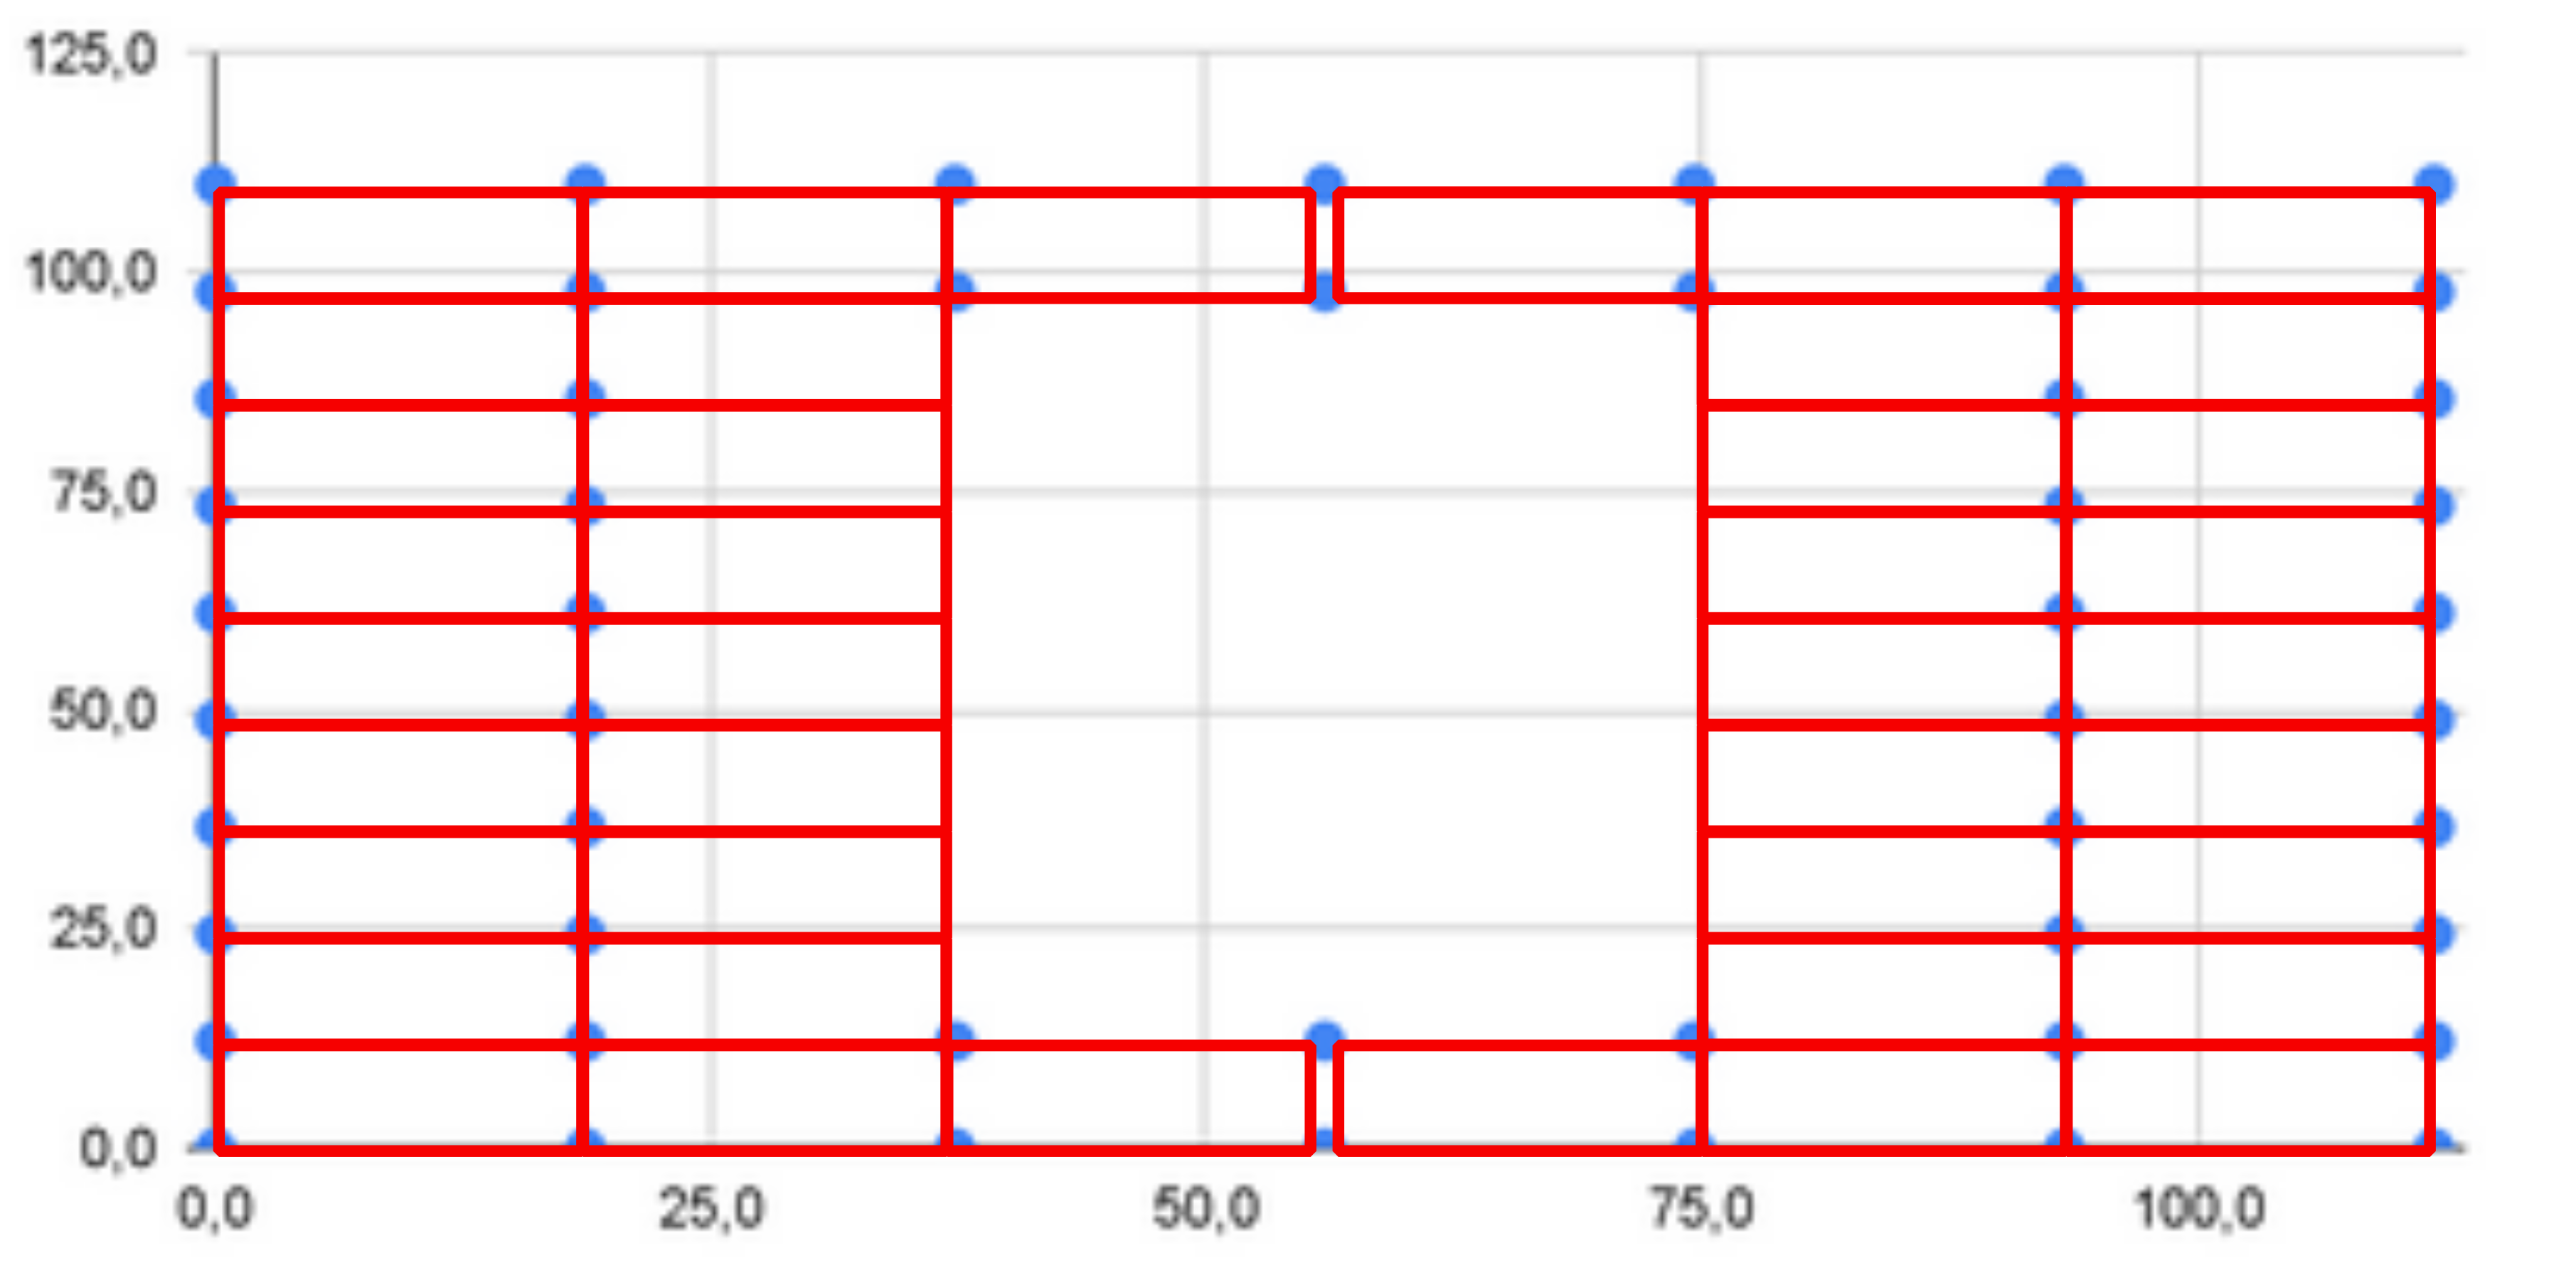
\includegraphics{grapheHV}\\ \\
\textsc{notes :} les formats supportés par le compilateur \texttt{pdflatex} sont le \textbf{.png, .jpg, .jpeg et .pdf}. On peut inclure des fichier sans pertes (\textbf{.svg}), on passe par une conversion en .pdf. De plus, pas besoin de préciser le type du fichier pour le lier au document (à part cas d'homonymie).

\section{Chemin d'accès}

Par défaut, le fichier est recherché dans le dossier où est placé le fichier \LaTeX. Cependant, on peut entrer un chemin à la place du simple nom du fichier.\\
On peut aussi définir un répertoire (dossier) à parcourir avec la commande \textit{\textbackslash graphicspath\{\{chemindudossier/\}\}}. Par ailleurs, chaque chemin se termine par un /. 

\section{Taille de l'image}

L'idéal est d'avoir une image à la taille voulue dès le départ. Cependant, il existe des façons de la redimensionner, avec les commandes fournie par la bibliothèque : \\

\begin{itemize}
\item \textit{\textbackslash includegraphics[width=largeur] \{nom du fichier\} }pour fixer la largeur
\item \textit{\textbackslash includegraphics[height=hauteur] \{nom du fichier\} }pour fixer la hauteur
\item \textit{\textbackslash includegraphics[scale=échelle] \{nom du fichier\} }pour fixer l'échelle\\
\end{itemize}

\textsc{notes :}la hauteur et la largeur sont définies en \texttt{cm}, l'échelle n'a pas d'unité. Par rapport à la grosseur, on multiplie ou on divise l'échelle par $\sqrt{2}$ (ex : on multiplie par 1.4 pour obtenir du A3 à partir du A4, par 2 pour multiplier la largeur par deux, passant de A4 à A2).

\section{Encadrement}

On peut inclure l'image dans un cadre en utilisant la commande \textit{\textbackslash fbox}.

\section{Figure flottante}

Tout camme avec les tableaux, on peut laisser le tupographe se charger de la disposition de l'image sur la page. Pour cela, on utilise l'environnement \textbf{figure}, couplé avec [position]. Dans l'exemple suivant, on a mis la largeur de l'image à \texttt{5cm} : \\ \\

\begin{figure}[h]
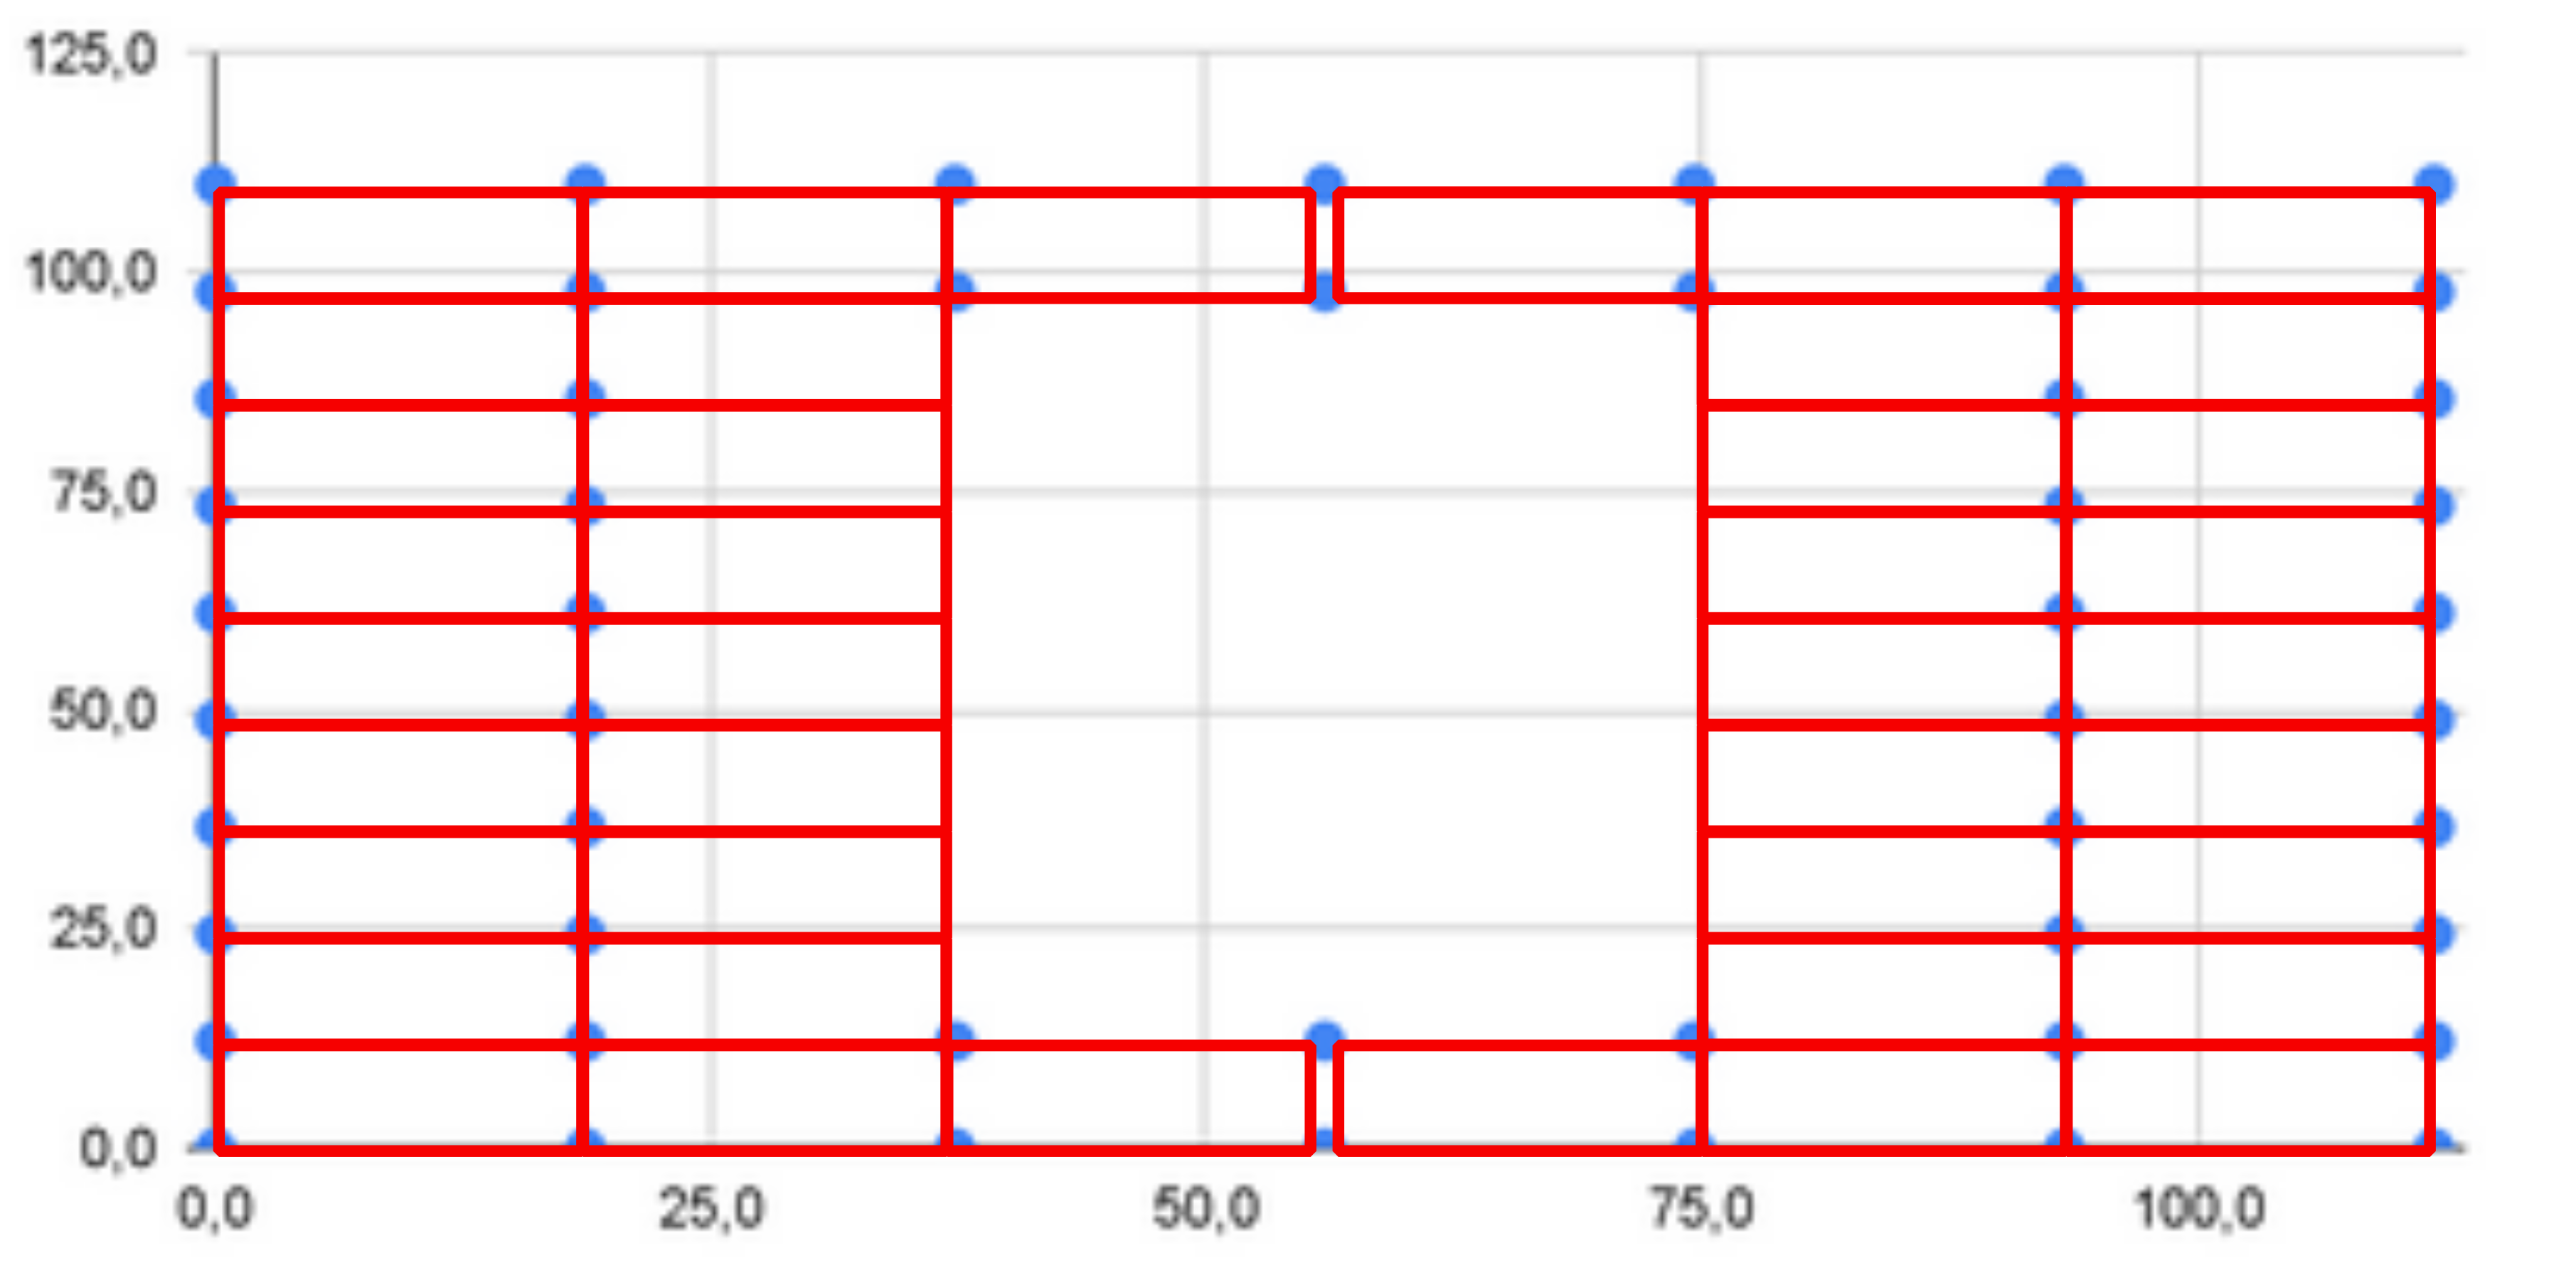
\includegraphics[width=5cm]{grapheHV}
\end{figure}

Pour rappel, voici les positions différentes proposées : \\ \\

\begin{itemize}
\item \texttt{h} pour que l'image soit à côté du texte la précédent (here)
\item \texttt{t} pour la placer en haut de la page
\item \texttt{b} pour la placer en bas de la page
\item \texttt{p} pour la mettre dans une page de flottants
\end{itemize}

\textsc{notes :}\LaTeX tient compte des règles internes de mise en page en priorité pour positionner une image. Pour forcer le positionnement d'une image, il faut précéder la lettre de position par un \textbf{!} (par exemple \textit{[!h]}. \\ On peut aussi insérer une légende, comme avec les tableaux.

\backmatter

\bibliographystyle{plain-fr}
\bibliography{mabiblio}

\tableofcontents

\end{document}